\chapter{Ray tracing on phase space} \label{chap:PS}
Ray tracing on phase space is a method which employs the phase space (PS) of the source and the target of the optical system.
Moreover, it takes into account the trajectory that every ray follows during its propagation.
Before explaining the method, we introduce the PS concept.
\section{Phase space}\label{sec:PSconcept}
Every ray in three dimensions is described by three position coordinates and three direction coordinates. 
The PS of an optical surface is characterized by two position and two direction coordinates, thus the PS of a three-dimensional systems is a four-dimensional space. The position coordinates are two of the coordinates of the intersection point of the ray with the surface of which we want to consider the PS, while the direction coordinates are the momentum coordinates of the vector tangent to the ray projected on that optical surface \cite{wolf2004geometric}.
\\ \indent 
In two dimensions, every ray parametrization is obtained from two position and two direction coordinates. The PS of an optical line is described by one position and one direction coordinate. Hence, for two-dimensional systems, every ray in PS is described by a point in a two-dimensional space.
Given an optical line $\lineai$, the ray position coordinate on PS is the $\variabile{x}$-coordinate of the intersection point between the ray and the line $\lineai$. The direction coordinate is the sine of the angle that the ray forms with respect to the normal \vect{$\boldsymbol{\nu}$} of line $\lineai$ multiplied by the index of refraction \n. We choose \vect{$\boldsymbol{\nu}$} always directed inside the same medium in which the incident ray travels. The PS is indicated with \set{S}{}{}$=$\set{Q}{}{}$\times$\set{P}{}{},
where \set{Q}{}{} is the set of the position coordinates \variabile{q} and \set{P}{}{} is the set of the direction coordinates $\variabile{p}=\variabile{n}\sin{\myangle}$, with $\myangle\in[-\pi/2, \pi/2]$ the angle between the ray segment inside the system and the normal measured counterclockwise.
In the following, the PS is considered only for the source $\point{S}$ and the target $\point{T}$ and for no other line of the optical system.
The coordinates of every ray on \set{S}{}{} and \set{T}{}{} are indicated with $(\variabile{q}_1,\variabile{p}_1)$ and $(\variabile{q},\variabile{p})$, respectively.\\ \indent
\begin{figure}[h]
  \begin{minipage}[]{0.49\textwidth}
\centering
    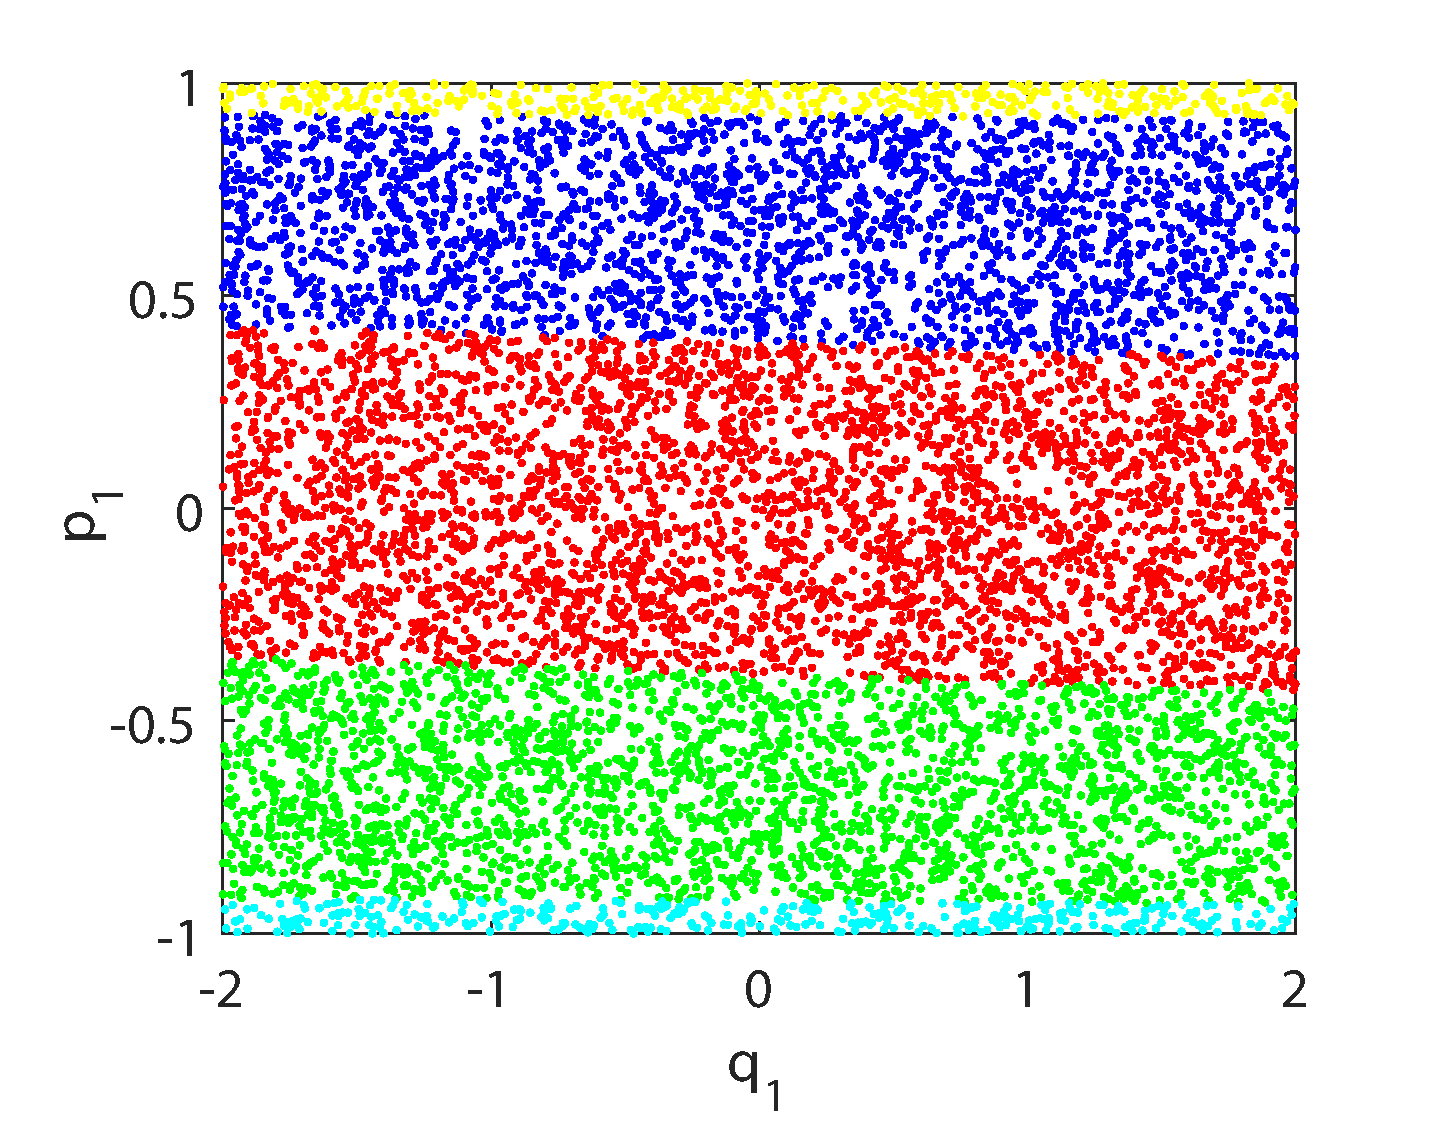
\includegraphics[width  = \textwidth]{source_PS_cup.pdf}
    \caption{Source PS of the two-faceted cup. Five different paths can occur.}
    \label{fig:sourcePS1}
  \end{minipage}
\hspace{0.2cm}
  \begin{minipage}[]{0.49\textwidth}
\centering
    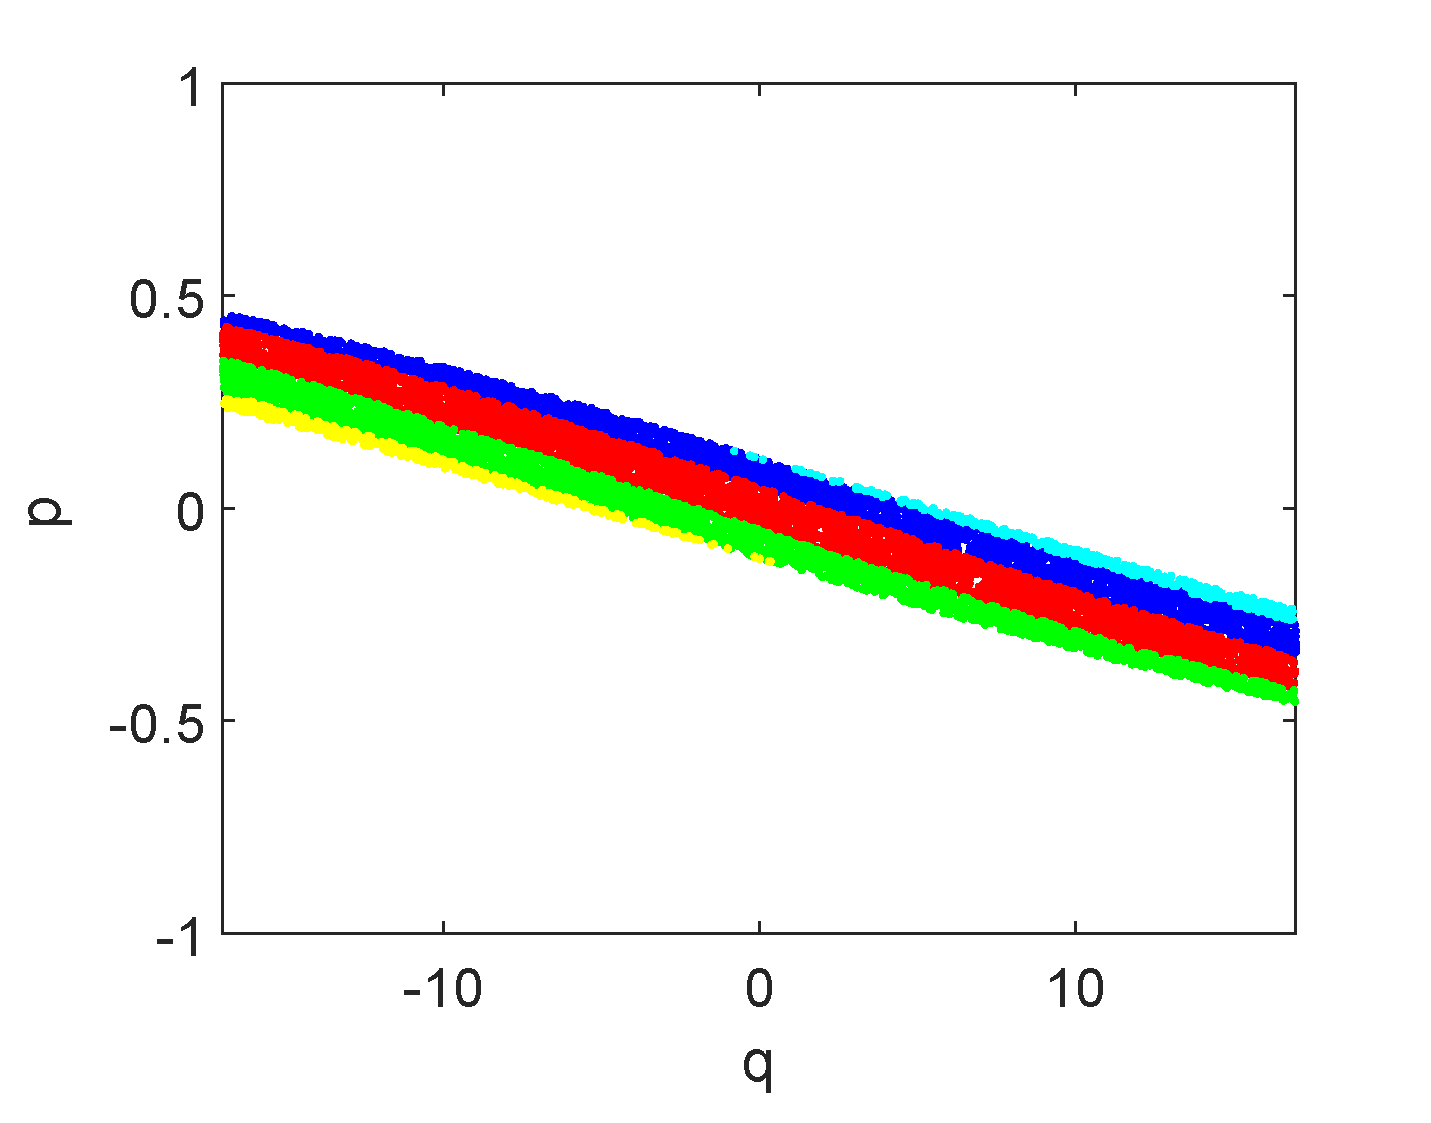
\includegraphics[width=\textwidth]{target_PS_cup.pdf}
  \caption{Target PS of the two-faceted cup. Five different paths can occur}
   \label{fig:targetPS1}
 \end{minipage}
\end{figure}
As an example, in Figures \ref{fig:sourcePS1} and \ref{fig:targetPS1} we show the source and target PS of the two-faceted cup (in Figure \ref{fig:cup}), sampled with $10^4$ random rays. The coordinates of every point correspond to the position and direction coordinates of a ray which are calculated using the ray tracing procedure. Furthermore, we store the path $\Pi$ that every ray follows, where we refer to a path as the sequence of lines encountered by the ray.
In Figures \ref{fig:sourcePS1} and \ref{fig:targetPS1} a color is associated to every path, hence all the rays that follow the same path are depicted with the same color.
We note that the source and target phase spaces are partitioned into different regions according to the path $\Pi$ followed by the rays.
Given a path $\Pi$, the corresponding regions are indicated with \set{R}{\textrm{s}}{}$(\Pi)$ and \set{R}{\textrm{t}}{}$(\Pi)$ at the source and the target PS, respectively.
Rays that propagate through the two-faceted cup can follow $5$ different paths. Some rays are emitted from the source and arrive at the target without hitting any other line, they follow path $\Pi_1= (1,4)$. These rays are depicted in red in the PS pictures. Some other rays can hit the left or the right reflector (line $2$ and $3$, respectively) once, their corresponding paths are $\Pi_2 = (1,2,4)$ and $\Pi_3 = (1,3,4)$, respectively. These rays are the blue and green dots in PS. Finally, there is the possibility that the rays have two reflections before hitting the target. They follow either path $\Pi_4 = (1,2,3,4)$ or path $\Pi_5 = (1,3,2,4)$ and they are depicted with the yellow and cyan points.
\\ \indent For the two-faceted cup all light emitted by the source arrives at the target. In order to derive the photometric variables at the target we need to understand where light ends up, i.e. which parts of the target PS are illuminated by the source. Indeed, while the source PS is completely covered by rays, some parts of the target PS are not reached by any ray at all, that is 
\begin{equation}
\begin{aligned}
\mbox{\set{S}{}{}} &= \bigcup_{\Pi} \mbox{\set{R}{\textrm{s}}{}}(\Pi),\\
\mbox{\set{T}{}{}} &\supset \bigcup_{\Pi} \mbox{\set{R}{\textrm{t}}{}}(\Pi),
\end{aligned}
\end{equation}
where the unions are over all the possible paths.
This means that, while the luminance at the source PS is positive for any possible position and direction, the luminance at the target PS is positive only inside the regions \set{R}{\textrm{t}}{}$(\Pi)$, for every path $\Pi$, and it is equal to $0$ outside those regions. For this reason, from now on we will refer to \set{R}{\textrm{t}}{}$(\Pi)$ as the \textit{positive luminance regions}. \\ \indent
It is very important to remark that, although \set{S}{}{} and \set{T}{}{} have a different ray distribution, the area covered by the rays is conserved. This follows from \'{e}tendue conservation. From (\ref{etendue2d}) we rewrite the two-dimensional \'{e}tendue as:
\begin{equation}
U = \int_{\variabile{x}^{\textrm{min}}}^{\variabile{x}^{\textrm{max}}} \int_{\myangle^{\textrm{min}}}^{\myangle^{\textrm{max}}} \n \cos(\myangle)\textrm{d}\variabile{x}\textrm{d}\myangle= \int_{\mbox{\set{Q}{}{}}}\int_{\mbox{\set{P}{}{}}} \textrm{d}\variabile{q}\,\textrm{d}\variabile{p}.
\end{equation}
where we indicated with $\variabile{x}^{\textrm{min}}$ and $\variabile{x}^{\textrm{max}}$ the minimum and maximum rays position coordinates and with $\myangle^{\textrm{min}}$ and $\myangle^{\textrm{max}}$ the minimum and maximum angles of the rays and the normal to the target. The second equality holds since $\textrm{d}\variabile{p}= \n\cos \myangle\textrm{d}\myangle$.
Therefore, in two dimensions, \'{e}tendue can be seen as an area in PS. Etendue conservation leads to the conservation of the areas of regions with positive luminance.\\ \indent
For the two-faceted cup in Figure \ref{fig:cup}, \set{S}{}{}$= [-2,2]\times[-1,1]$, thus, the \'{e}tendue at the source is $U_\textrm{s}=8$ (see Figure \ref{fig:sourcePS1}). Computing the total area covered by the positive luminance regions at the target using the trapezoidal rule, we obtain $U_\textrm{t}=8$ which numerically proves \'{e}tendue conservation for the two faceted-cup. 
From this follows a fundamental principle in non-imaging optics which is referred to as "the edge-ray principle". A literature overview of this principle is given in the next paragraph.
\section{The edge-ray principle}
The goal in non-imaging optics is to transfer all light from the source aperture to the output aperture. Systems that satisfy this property are referred to \textit{ideal optical systems}.
Several methods to design ideal optical systems are based on the edge-ray principle, \cite{welford1978problem, benitez1997design}. 
Basically it states that all the light rays exiting the edges of the source will end at the edges of the target. 
This guarantees that all light emitted from the source will arrive at the receiver, see Figure \ref{fig:edge}. 
 \begin{figure}[h]
  \begin{center}
  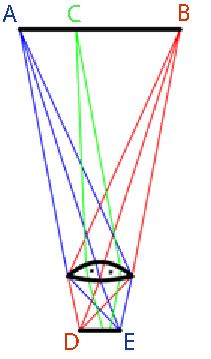
\includegraphics[width= 3.5cm]{Edge-ray}
  \end{center}
  \caption{A lens receiving light from a source $\textrm{A}\textrm{B}$ and redirects it to the receiver $\textrm{D}\textrm{E}$. 
Rays that leave the edges of the source hit the edges of the target (blue and red rays). Rays coming from the interior of the source will end at the interior of the target (green rays) \cite{wiki2}.}
  \label{fig:edge}
\end{figure}
\\ \indent
In $1985$ Mi{\~n}ano proved the principle by using the PS of the source and the target of an optical system, \cite{minano1985two, minano1986design}. He proved the principle for systems in inhomogeneous media, where the index of refraction is a continuous function, so the map that connects the source and target phase spaces is a continuous map.
Indicating with $\map{M}{}{}(P)$ the optical map of a point $P$, Mi{\~n}ano showed that if $\map{M}{}{}(\partial\mbox{\set{S}{}{}})=\partial\mbox{\set{T}{}{}}$ then 
$\map{M}{}{}(\mbox{\set{S}{}{}})=\mbox{\set{T}{}{}}$ and vice versa. 
%Note that the trajectory of two rays in PS cannot cross. 
The first version of the edge-ray principle \cite{minano1986design} can be enunciated in two-dimensions as follows:
\begin{lemma}{Edge-ray principle (version1)}\\ 
Suppose that:
\begin{itemize}
\item[a)] There are two regions \set{R}{\textrm{s}}{} and \set{R}{\textrm{t}}{} in source and target PS with the same area such that 
$$\map{M}{}{}(\partial\mbox{\set{R}{\textrm{s}}{}}) = \map{M}{}{}(\partial\mbox{\set{R}{\textrm{t}}{}});$$ 
\item[b)] The refractive-index distribution $\n$ is a continuous function; 
%\item[c)] They have the direction cosine with respect to the optical axis greater than $0$;
\end{itemize}
Then, the following relation holds: $$\map{M}{}{}(\mbox{\set{R}{\textrm{s}}{}}) = \map{M}{}{}(\mbox{\set{R}{\textrm{t}}{}}).$$
\end{lemma} 
The previous lemma claims that if there exist a map connecting the boundaries of two regions from the source to the target, then also the interior of those regions are connected using the same map. Note that the second assumption in the previous lemma implies that the optical map is continuous in PS.
However, for some optical systems, as for instance the compound parabolic concentrator (CPC), the ray mapping in PS is not continuous. This is due to multiple reflections that rays can encounter with the reflectors and implies that some rays at the edge of the source could not be mapped into rays at the edges of the target \cite{davies1994edge}. \\ \indent 
In 1994 Ries and Rabl reformulated the edge-ray principle such that it is valid for all systems even if the ray map in PS is not continuous \cite{Ries:2}. 
Suppose that \set{R}{\textrm{s}}{}$(\Pi)$ and \set{R}{\textrm{t}}{}$(\Pi)$ are the regions, corresponding to path $\Pi$, at the source and the target PS, respectively. 
They showed that, for a given path $\Pi$, if the boundaries
$\partial$\set{R}{\textrm{s}}{}$(\Pi)$ are mapped into the boundaries $\partial$\set{R}{\textrm{t}}{}$(\Pi)$, then also the regions \set{R}{\textrm{s}}{}$(\Pi)$ are mapped into the regions \set{R}{\textrm{t}}{}$(\Pi)$.
Then, to map \set{S}{}{} to \set{T}{}{} it is necessary and sufficient that the first version of the edge ray principle is observed for all part of \set{S}{}{} and \set{T}{}{} defined by the number of reflections \cite{Ries:2}. 
\begin{lemma}{Edge-ray principle (generalized version)}\\
Let indicate every possible path with $(\Pi_\variabile{j})_{\variabile{j}=1, \cdots, \npath}$, where $\npath$ is the number of all possible paths.
Every possible path correspond to a certain number of reflections or refraction.
Let denote with \set{R}{\textrm{s}}{}$(\Pi_\variabile{j})$ and \set{R}{\textrm{t}}{}$(\Pi_\variabile{j})$ the regions at \set{S}{}{} and \set{T}{}{} associated to path $\Pi_\variabile{i}$ such that they are a partition of \set{S}{}{} and \set{T}{}{}, that is:
\begin{equation*}
\begin{aligned}
\mbox{\set{S}{}{}} &= \bigcup_{\variabile{j}=1}^{\npath} \mbox{\set{R}{\textrm{s}}{}}(\Pi_\variabile{i}), \mbox{ with } \mbox{\set{R}{\textrm{s}}{}}(\Pi_\variabile{j})\cap \mbox{\set{R}{\textrm{s}}{}}(\Pi_\variabile{i}) = \emptyset \mbox{ for } \variabile{i}\neq \variabile{j}\\
\mbox{\set{T}{}{}} & \supset \bigcup_{\variabile{j}=1}^{\npath} \mbox{\set{R}{\textrm{t}}{}}(\Pi_\variabile{i}), \mbox{ with } \mbox{\set{R}{\textrm{t}}{}}(\Pi_\variabile{j})\cap \mbox{\set{R}{\textrm{t}}{}}(\Pi_{\variabile{i}}) = \emptyset \mbox{ for } \variabile{j}\neq \variabile{i}.
\end{aligned}
\end{equation*} 
Then, to map a source region into a target, it is necessary and sufficient that the first version of the edge ray principle is observed for all parts of \set{S}{}{} and \set{T}{}{}: 
\begin{equation*}
\map{M}{}{}\big(\partial\mbox{\set{R}{\textrm{s}}{}}(\Pi_{\variabile{j}})\big) = \partial\mbox{\set{R}{\textrm{t}}{}}(\Pi_{\variabile{j}}), \quad \forall \variabile{j}\in\{1, \cdots, \npath\}.
\end{equation*}
\end{lemma}
Hence, the edge-ray principle constitutes a tool for designing ideal systems and, to this purpose, it is sufficient that the rays of $\partial$\set{R}{\textrm{s}}{}$(\Pi)$ are transformed to the rays of $\partial$\set{R}{\textrm{t}}{}$(\Pi)$ for every path $\Pi$ \cite{minano1992new}. 
\\ \indent Using the PS concept and the edge-ray principle we develop a new ray tracing method. 
A non-uniform distribution of the rays is provided by developing a triangulation refinement at the source PS which is explained in the next section. 
The triangulation refinement provides more rays close to the boundaries of the regions \set{R}{\textrm{s}}{}$(\Pi)$ each of them is formed by the rays that follow the same path $\Pi$.
%Next, the boundaries $\partial$\set{R}{\textrm{s}}{}$(\Pi)$ are approximated by using two different approaches that will be explained Chapter \ref{chap:boundaries_alpha} and Chapter{}. For every path $\Pi$, the boundaries at the target $\partial$\set{R}{\textrm{t}}{}$(\Pi)$ are obtained by mapping their corresponding boundaries $\partial$\set{R}{\textrm{s}}{} at the source.
\section{Phase space ray tracing}\label{sec:PS_raytracing}
PS ray tracing takes advantage of the fact that there exists an optical map
$
\map{M}{}{}: \mbox{\set{S}{}{}} \mapsto \mbox{\set{T}{}{}}
$
 such that
\begin{equation}\label{eq:map1}
\map{M}{}{}(\variabile{q}_1,\variabile{p}_1)=(\variabile{q},\variabile{p}),
\end{equation} for every $(\variabile{q}_1,\variabile{p}_1)\in$ \set{S}{}{}.
For very simple systems, like the two-faceted cup, it is possible to determine an analytic expression for $\map{M}{}{}$ (as explained in Appendix \ref{app:boundariescup}).
This is not the case for most of the optical systems we deal with. In these cases it is necessary to implement ray tracing to calculate how light is distributed at the target.
As mentioned in the previous paragraph, for some optical systems $\map{M}{}{}$ is not even continuous.
Nevertheless, given a path $\Pi$, the restriction of $\map{M}{}{}$ to \set{R}{\textrm{s}}{}$, i.e., \map{M}{}{}(\Pi)$: \set{R}{\textrm{s}}{}$(\Pi)$ $\mapsto$ \set{R}{\textrm{t}}{}$(\Pi)$ is a continuous and bijective map. 
The edge ray principle guarantees that $\map{M}{}{}(\Pi)$ maps \set{R}{\textrm{s}}{}$(\Pi)$ onto \set{R}{\textrm{t}}{}$(\Pi)$ preserving topological features. In particular, the boundary $\partial$\set{R}{\textrm{s}}{}$(\Pi)$ is mapped onto the boundary $\partial$\set{R}{\textrm{t}}{}$(\Pi)$. %, see \cite{Ries, Davies, Minano}.
Employing the maps $\map{M}{}{}(\Pi)$ for all the possible paths $\Pi$, the output light distribution is determined. Therefore, the photometric variables at the target can be calculated.
\\ \indent The luminance $L(\variabile{q}, \variabile{p})$ at the target PS is given by:
\begin{equation}
\begin{aligned}
\label{eq:PSluminance}
L(\variabile{q}, \variabile{p}) &> 0  \mbox{  for } (\variabile{q}, \variabile{p})\in \mbox{\set{R}{\textrm{t}}{}}(\Pi) \mbox{ for some path } \Pi,\\ \vspace{0.5 cm}
L(\variabile{q}, \variabile{p}) &= 0  \mbox{  otherwise}.
\end{aligned}
\end{equation}
The target intensity along a given direction $\variabile{p}=\const{const}$ is computed through an integration of the target luminance $L(\variabile{q}, \variabile{p})$ over $\variabile{q}$ and it is defined in \set{T}{}{}$\,$ by:
\begin{equation}
\label{eq:PSintensity}
I_{\textrm{PS}}(\variabile{p}) = \int_{\mbox{\set{Q}{}{}}}L(\variabile{q}, \variabile{p}) \textrm{d}\variabile{q}.
\end{equation}
Note that, while in the real space the intensity is defined as a function of the angular coordinate $\myangle$ (see Chapter \ref{chap:Illumination optics}), in PS the intensity is defined as a function of the direction coordinate $\variabile{p}=\n\sin(\myangle)$.
The previous equation implies that, assuming a Lambertian source, the problem of computing the target intensity is reduced to the problem of calculating the boundaries
$\partial$\set{R}{\textrm{t}}{}$(\Pi)$ for all possible paths $\Pi$. Hence, the intensity along the direction $\variabile{p}= \textrm{const.}$ is given by the sum of the interval lengths formed by the support of the luminance and line $\variabile{p}=\textrm{const.}$. For example, if two intersection points between line $\variabile{p}= \textrm{const.}$ and the boundary $\partial$\set{R}{\textrm{t}}{}$(\Pi)$ are found, indicating their position coordinates with $\variabile{q}^\textrm{min}(\Pi,\variabile{p})$ and $\variabile{q}^\textrm{max}(\Pi,\variabile{p})$, where $\variabile{q}^\textrm{min}(\Pi,\variabile{p})<\variabile{q}^\textrm{max}(\Pi,\variabile{p})$, and using Equation (\ref{eq:PSluminance}), we obtain that Equation (\ref{eq:PSintensity}) reduces to:
\begin{equation}\label{eta2}
I_{\textrm{PS}}(\variabile{p}) = \sum_{\Pi}\int_{\variabile{q}^\textrm{\,min}(\Pi, \variabile{p})}^{\variabile{q}^\textrm{\,max}(\Pi,\variabile{p})}L(\variabile{q}, \variabile{p})\textrm{d}\variabile{q} = \sum_{\Pi}\big (\variabile{q}^\textrm{max}(\Pi,\variabile{p})-\variabile{q}^\textrm{\,min}(\Pi,\variabile{p})\big )\,,
\end{equation}
where the sum is over all the possible paths and the second equation holds as we assume Lambertian source with $L=1$ in \set{R}{\textrm{t}}{}($\Pi$). In case more then two intersection points occur, a generalized equation needs to be used for calculating the intensity. 
Note that for every single ray only one path is possible as we are assuming that all the lines are reflective lines.
Because of this, the regions \set{R}{\textrm{t}}{}($\Pi$) do not overlap, i.e.
\begin{equation}
\bigcap_{\Pi}\mbox{\set{R}{\textrm{t}}{}}(\Pi)= \emptyset,
\end{equation}
where the intersection is over all possible paths. \\ \indent
From Equation (\ref{eta2}) we note that, using the PS structure, only the rays on the boundaries $\partial$\set{R}{\textrm{t}}{}$(\Pi)$ are required for obtaining the target intensity profile.
%Instead of tracing the rays randomly (as in MC ray tracing) or following a regular source distribution (as in QMC ray tracing)
The aim is to construct a ray tracing procedure that allows us tracing less rays overall and more rays close to the discontinuity of the luminance, i.e. close to the boundaries $\partial$\set{R}{\textrm{t}}{}$(\Pi)$.
To this purpose, we start from a triangulation made by only two triangle, then a triangulation refinement at \set{S}{}{} is defined as explained in the following. \\ \indent
The procedure starts with coordinates $(\variabile{q}_1^\variabile{k},\variabile{p}_1^\variabile{k})_{\variabile{k}=1, \cdots, 4}$ of the four corner points of \set{S}{}{}. For each of them, the corresponding path $(\Pi^\variabile{k})_{\variabile{k}=1, \cdots, 4}$ is calculated. Next, the grid is divided into two equal triangles joining two opposite vertices (in our simulation we always trace the diagonal north-west to define the new triangles). For each triangle the rays located at its corners are traced. If the paths corresponding to
those rays are not all equal, one or more boundaries
$\partial$\set{R}{\textrm{t}}{}$(\Pi)$ are expected to cross the triangle.
In that case, the middle points $(\variabile{q}_1^\variabile{k},\variabile{p}_1^\variabile{k})_{\variabile{k}=5,6,7}$ of each side of the triangle are added and
the three corresponding rays are traced (unless they were already traced in the previous steps). Each refinement step leads to four new triangles (see Figure \ref{fig:refinement}).
 \begin{figure}[h]
 \begin{minipage}[h]{\textwidth}
\centering
    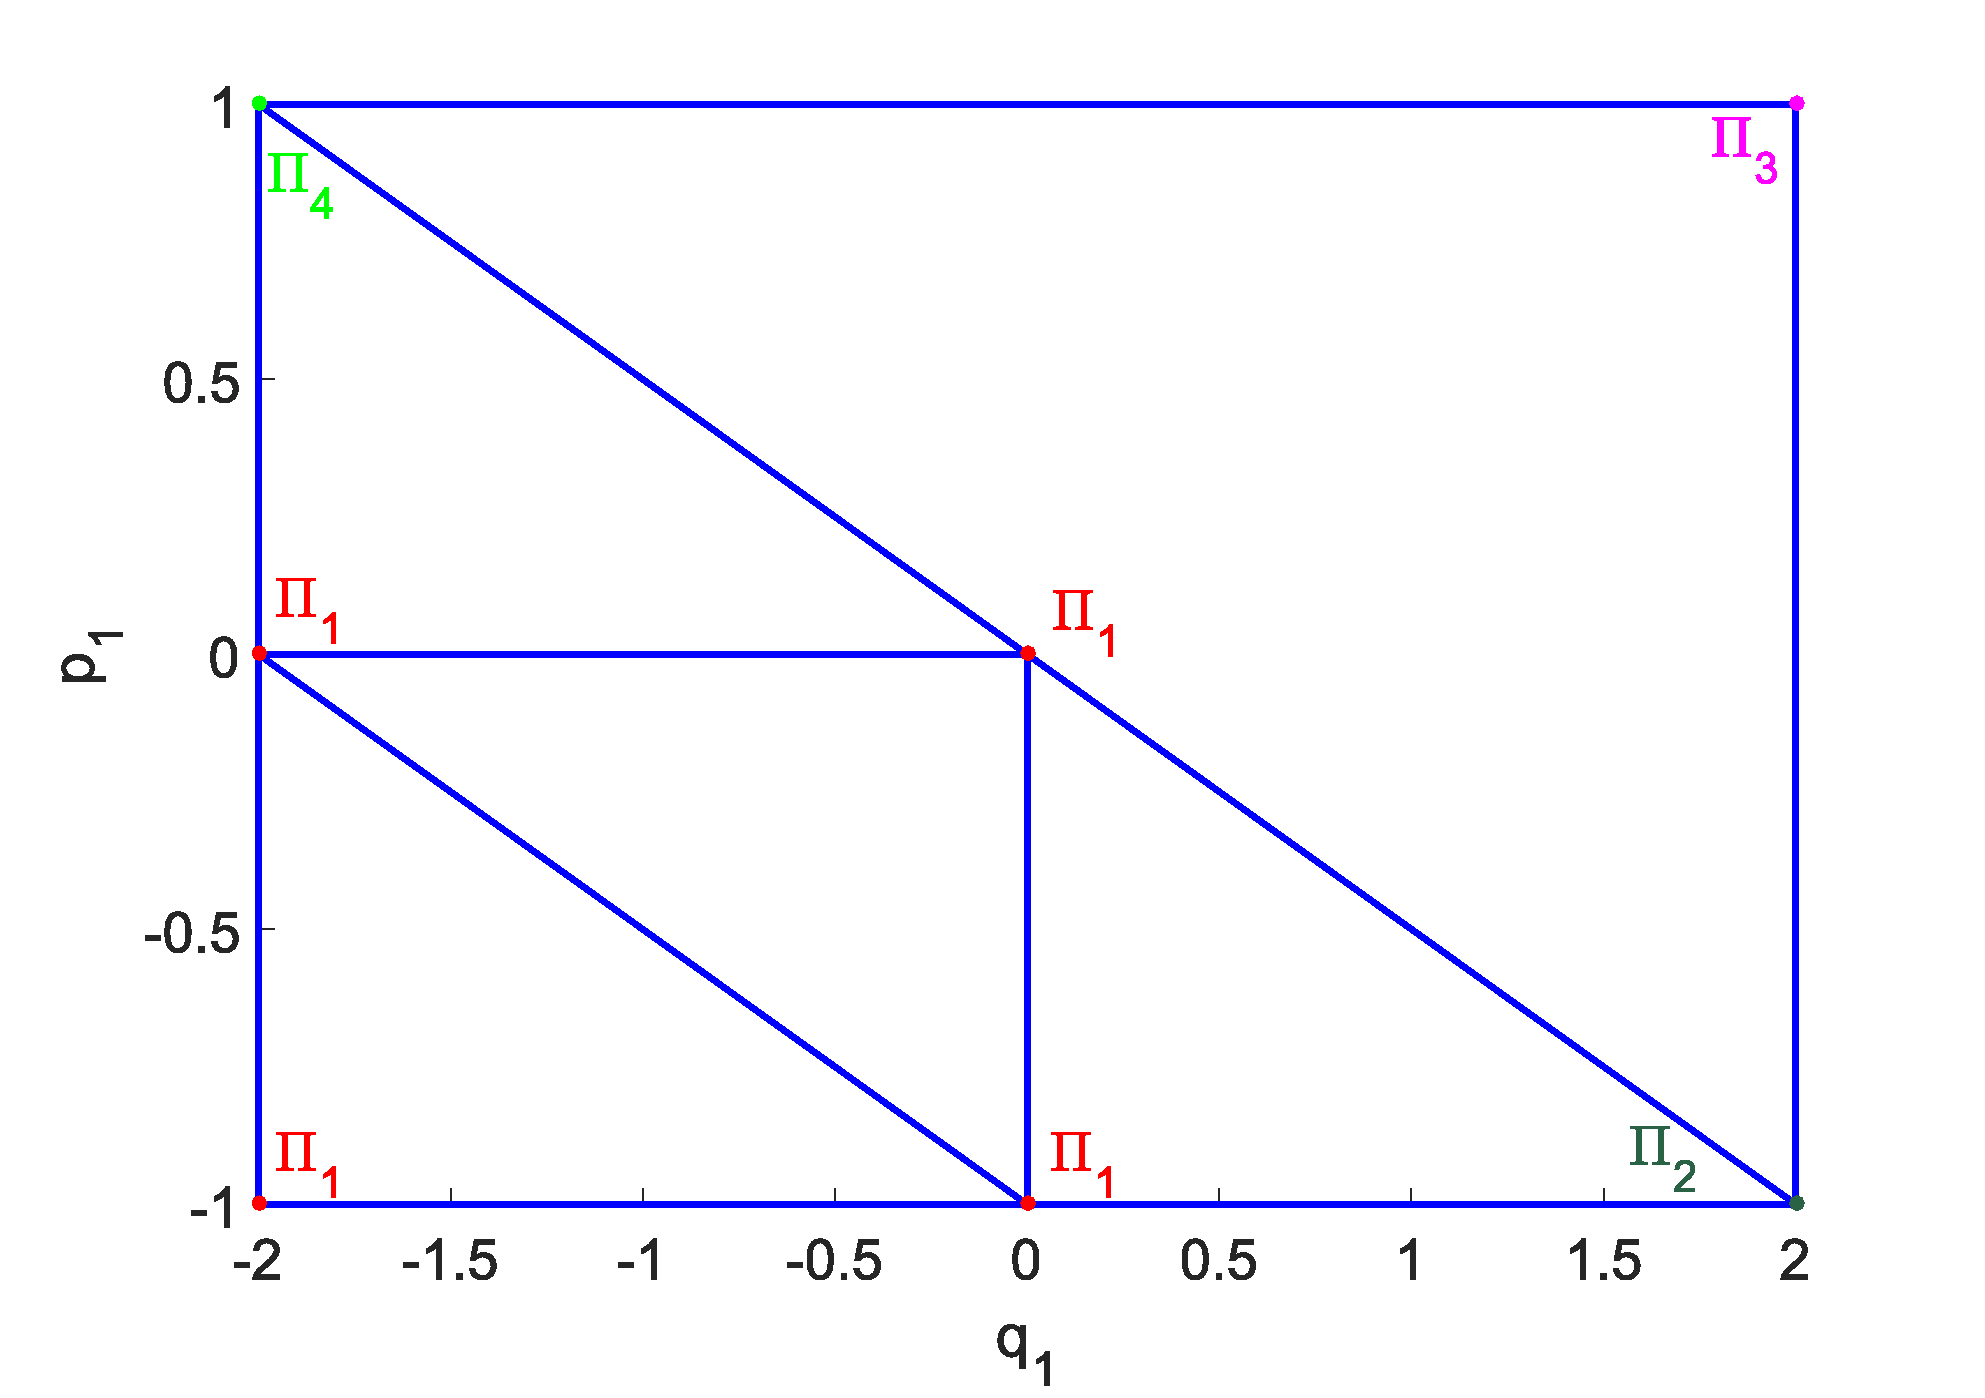
\includegraphics[width  = 0.9\textwidth]{region}
  \caption{Triangulation refinement:
  when the rays related to the vertices of the triangles follow a different path a new refinement step is required.
   Each refinement step leads to four new triangles.}
   %The parameters values are $\varepsilon_{\variabile{q}_{max}}~=~ 2$, $\varepsilon_{\variabile{p}_{max}}= 1$, $\varepsilon_{\variabile{q}_{min}}= 4$ and $\varepsilon_{\variabile{p}_{min}}=2$.}
  \label{fig:refinement}
\end{minipage}\\
\begin{minipage}[h]{\textwidth}
\centering
    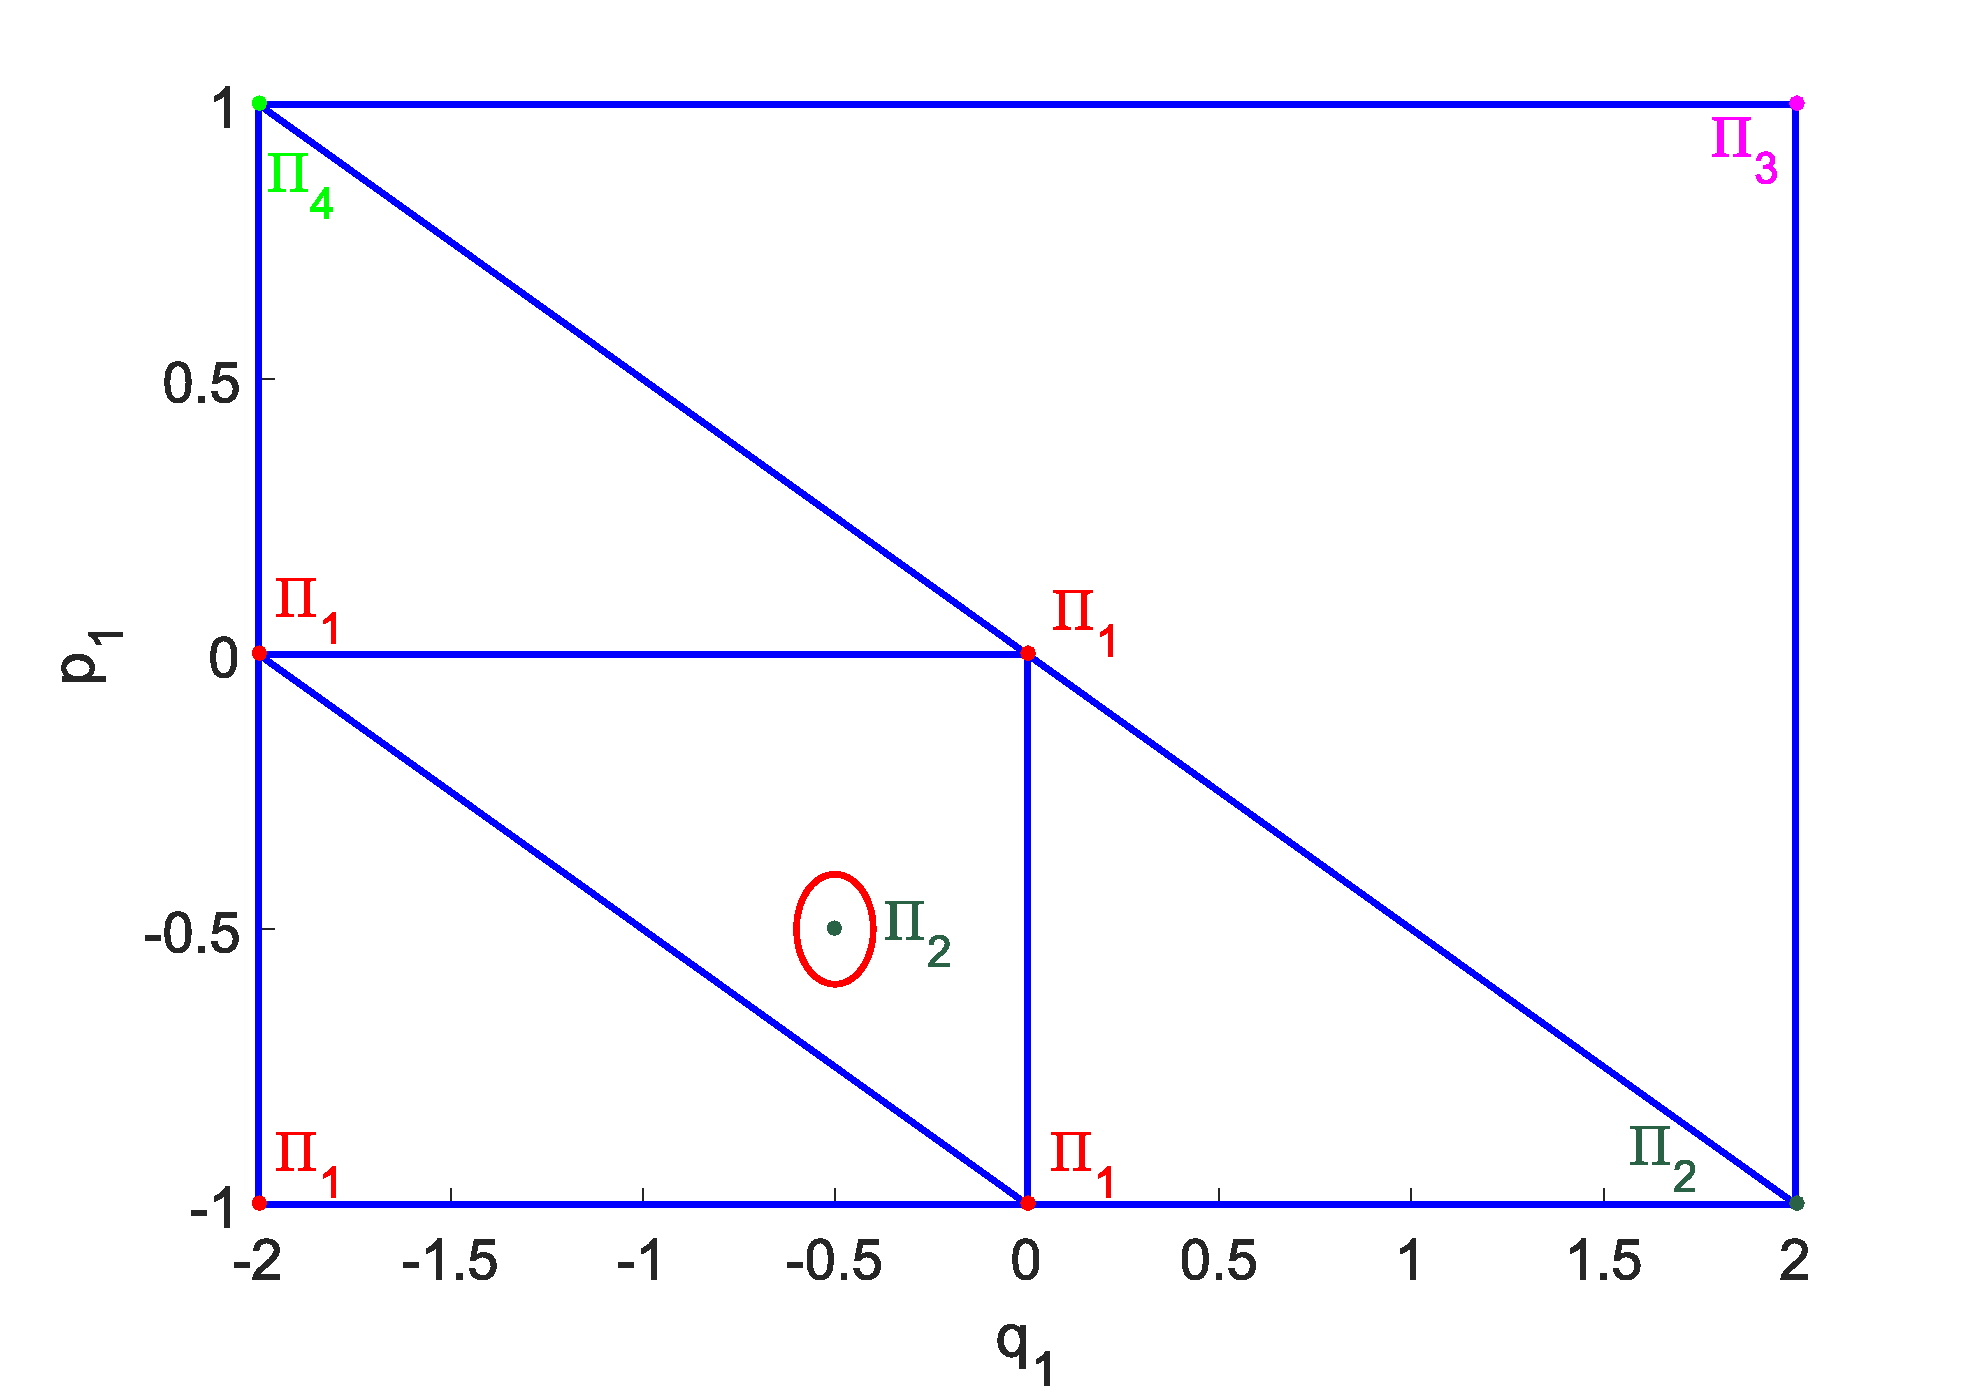
\includegraphics[width  = 0.9\textwidth]{region_inside}
  \caption{The red line encloses a region of rays that follow the path $\Pi_2$ and is completely located inside a triangle.
  The algorithm is not able to detect that region and, a further refinement is required.}
   \label{fig:region inside}
\end{minipage}
  \end{figure} \\ \indent
When all the rays corresponding to the corners of each triangle have the same path, it is not necessary to refine the triangles anymore.
Since the triangles very close to the boundaries are always crossed by at least a boundary, at least two different paths are found for the rays at the vertices of those triangles. 
Because of this, the procedure could continue infinitely, therefore, two parameters $\varepsilon_\variabile{q}^\textrm{min}$ and $\varepsilon_\variabile{p}^\textrm{min}$ are introduced to defined a stopping criterion.
The algorithm stops when the length of the sides of the triangles is smaller than $\varepsilon_\variabile{q}^\textrm{min}$ and $\varepsilon_\variabile{p}^\textrm{min}$ in $\variabile{q}$ and $\variabile{p}$ direction. \\ \indent 
We indicate all the possible paths with $(\Pi_{\variabile{j}})_{\variabile{j}=1, \cdots, \npath}$ where $\npath$ is the maximum number of paths\footnote{We remind the reader that we indicate with $\Pi^\variabile{k} = \Pi(\variabile{q}_1^\variabile{k},\variabile{p}_1^\variabile{k})$ the path followed by rays with coordinates $(\variabile{q}_1^\variabile{k},\variabile{p}_1^\variabile{k})$ in source PS. Note that it
can happen $\Pi^\variabile{k}= \Pi^\variabile{h}$ for $\variabile{k}\neq\variabile{h}.$
With $(\Pi_{\variabile{j}})_{\variabile{j}=1, \cdots, \npath}$ we indicate all the possible $\npath$ paths that can occur, therefore $\Pi_{\variabile{i}}\neq\Pi_{\variabile{j}}$ if $\variabile{i}\neq\variabile{j}$.} (\npath = 5 for the two-faceted cup).
If the size of the triangles is too big, it can happen that a region formed by rays that follow a path $\Pi_\variabile{j}$ is located completely inside a triangle whose vertices are related to another path $\Pi_\variabile{i}$ with $\variabile{j} \neq  \variabile{i}$, see Figure \ref{fig:region inside}.
To avoid this, two parameters $\varepsilon_\variabile{q}^{\textrm{max}}$ and $\varepsilon_\variabile{p}^{\textrm{max}}$ are defined for the $\variabile{q}_1$-axis and the $\variabile{p}_1$-axis, respectively.
When the length of the sides of the triangle are greater than these parameters, a new triangle is defined even if its vertices correspond to the same path.
The values of the parameters $\varepsilon_\variabile{q}^\textrm{min}$, $\varepsilon_\variabile{p}^\textrm{min}$, $\varepsilon_\variabile{q}^\textrm{max}$ and $\varepsilon_\variabile{p}^\textrm{max}$ determine the number of rays traced.
Thus, on the one hand, decreasing $\varepsilon_\variabile{q}^\textrm{min}$ and $\varepsilon_\variabile{p}^\textrm{min}$ more rays close to the boundaries are traced;
on the other hand, decreasing the values of $\varepsilon_\variabile{q}^\textrm{max}$ and $\varepsilon_\variabile{p}^\textrm{max}$ more rays in the interior of the regions are traced. \\ \indent The triangulation refinement is provided by Algorithm \ref{alg:triangulation} which uses the two recursive functions L$\footnotesize{\textrm{EFT}}$ T$\footnotesize{\textrm{RIANGLE}}$ and  R$\footnotesize{\textrm{IGHT}}$ T$\footnotesize{\textrm{RIANGLE}}$.
The function L$\footnotesize{\textrm{EFT}}$ T$\footnotesize{\textrm{RIANGLE}}$ is defined in Algorithm \ref{alg:left_triangle} (see Figure \ref{fig:triangulation_left}). 
A similar procedure gives the function R$\footnotesize{\textrm{IGHT}}$ T$\footnotesize{\textrm{RIANGLE}}$ (see Figure \ref{fig:triangulation_right}).
\begin{algorithm}[h]
\caption{Triangulation refinement algorithm}\label{alg:triangulation}
Initialize $\varepsilon_{\variabile{q}}^{\textrm{min}}, \varepsilon_{\variabile{q}}^{\textrm{max}}, \varepsilon_{\variabile{p}}^{\textrm{min}},$ and
 $\varepsilon_{\variabile{p}}^{\textrm{max}}$, Ray = [empty];\\
Define a structure that contains related data in fields. Each field can contain every type of data. \\
\Comment $\varepsilon_{\variabile{q}}^{\textrm{min}}, \varepsilon_{\variabile{q}}^{\textrm{max}}, \varepsilon_{\variabile{p}}^{\textrm{min}},$ and
 $\varepsilon_{\variabile{p}}^{\textrm{max}}$ are fixed parameters needed to stop the procedure\\
\Comment Ray: structure that contains all the data of rays traced (i.e., position, direction and path).
\begin{algorithmic}[1]
%\Procedure{Triangulation refinement}{}
\State $(\variabile{q}_1^1, \variabile{p}_1^1)= (-\variabile{a}, -1)$ \Comment \mbox{left bottom corner of source PS \;}
\State $(\variabile{q}_1^2, \variabile{p}_1^2) = (\variabile{a}, -1)$ \Comment \mbox{right bottom corner of source PS}
\State $(\variabile{q}_1^3, \variabile{p}_1^3)  = (\variabile{a}, 1)$ \Comment \mbox{right upper corner of source PS\;\;}
\State $(\variabile{q}_1^4, \variabile{p}_1^4) = (-\variabile{a}, 1) $ \Comment \mbox{left upper corner of source PS\;\;\;\;\,}
\For{$ \variabile{k}= 1 \to 4 $}
\State Trace the ray with initial coordinates $(\variabile{q}_1^\variabile{k}, \variabile{p}_1^{\variabile{k}})$ in \set{S}{}{};
\State Calculate the corresponding path $\Pi^{\variabile{k}}$; $\qquad \qquad \qquad \qquad \qquad \qquad \qquad \qquad\quad$
\Comment Store the information found in the structure Ray;
\State $\textrm{Ray}.\variabile{q}= [\mbox{Ray}.\variabile{q}, \variabile{q}_1^\variabile{k}]$;
\State $\textrm{Ray}.\variabile{p}= [\mbox{Ray}.\variabile{p}, \variabile{p}_1^\variabile{k}]$;
\State $\textrm{Ray}.\Pi = [\mbox{Ray}.\Pi, \Pi^{\variabile{k}}]$;
\EndFor
\State VL $= [1, 2, 4]$ \Comment{VL vertices of the left triangle\;\,\,\,}
\State VR $= [2,3, 4]$   \Comment{VR vertices of the right triangle}
\State \Call{Left Triangle}{VL, Ray, $\varepsilon_{\variabile{q}_1}^{\textrm{min}}, \varepsilon_{\variabile{q}_1}^{\textrm{max}}, \varepsilon_{\variabile{p}_1}^{\textrm{min}}, \varepsilon_{\variabile{p}_1}^{\textrm{max}}$}\Comment{Refine the left triangle\;\,\,} 
\State \Call{Right Triangle}{VR, Ray, $\varepsilon_{\variabile{q}_1}^{\textrm{min}}, \varepsilon_{\variabile{q}_1}^{\textrm{max}}, \varepsilon_{\variabile{p}_1}^{\textrm{min}}, \varepsilon_{\variabile{p}_1}^{\textrm{max}}$} \Comment{Refine the right triangle} \\
\Return Ray;
%\EndProcedure
\end{algorithmic}
\end{algorithm}
\begin{algorithm}[h]
\caption{Algorithm for the refinement of the left triangles}\label{alg:left_triangle}
\begin{algorithmic}[1]
\Procedure{Left triangle}{VL, Ray, $\varepsilon_{\variabile{q}}^{\textrm{min}}, \varepsilon_{\variabile{q}}^{\textrm{max}}, \varepsilon_{\variabile{p}}^{\textrm{min}}, \varepsilon_{\variabile{p}}^{\textrm{max}}$}
\State $\textrm{VL}= [1,2,4]$
\State $\variabile{q}_1^1= \textrm{Ray}.\variabile{q}(\textrm{VL}(1))$, $\variabile{p}_1^1= Ray.\variabile{p}(\textrm{VL}(1))$
\State $\variabile{q}_1^2= \textrm{Ray}.\variabile{q}(\textrm{VL}(2))$, $\variabile{p}_1^2= Ray.\variabile{p}(\textrm{VL}(2))$
\State $\variabile{q}_1^3= \textrm{Ray}.\variabile{q}(\textrm{VL}(3))$, $\variabile{p}_1^3= Ray.\variabile{p}(\textrm{VL}(4))$
\State $\textrm{dist}_\variabile{q}= \mbox{$|\variabile{q}_1^2-\variabile{q}_1^1|$}$
\State $\textrm{dist}_\variabile{p}= \mbox{$|\variabile{p}_1^{3}-\variabile{p}_1^1|$}$
\State RefineTriangle $=$  false;
\State DifferentPath $=$  false;
\If{$\textrm{dist}_\variabile{q}>\varepsilon_{\variabile{q}}^{\textrm{max}} $ or $\textrm{dist}_\variabile{p} >\varepsilon_{\variabile{p}}^{\textrm{max}}$}
\State RefineTriangle $=$  true;
\EndIf
\For{$ \variabile{k} = 1 \to 2 $}
\If{$\Pi^{\variabile{k}} \neq \Pi^{\variabile{k}+1}$}
\State DifferentPath $=$  true;
\EndIf
\EndFor
\If{$\textrm{dist}_\variabile{q}>\varepsilon_{\variabile{q}}^{\textrm{min}}$ or $\textrm{dist}_\variabile{p}>\varepsilon_{\variabile{p}}^{\textrm{min}}$}
\State RefineTriangle $=$  DifferentPath;
\Else
\If{(DifferentPath is true)}
\State Ray(\textrm{VL}).boundary $=$ true; \Comment{A boundary crosses the triangle}
\EndIf
\EndIf
\If {(RefineTriangle is true)}
\State Define the points at the middle of each side of the triangle
\State $(\variabile{q}_1^5, \variabile{p}_1^5) = ((\variabile{q}_1^1+\variabile{q}_1^2)/2, \variabile{p}_1^1)$
\State $(\variabile{q}_1^6, \variabile{p}_1^6) = (\variabile{q}_1^5, (\variabile{p}_1^1+\variabile{p}_1^2)/2)$
\State $(\variabile{q}_1^7, \variabile{p}_1^7) = (\variabile{q}_1^1, \variabile{p}_1^6)$
\For {$\variabile{k} = 5 \to 7 $}
\If {The ray with coordinates $(\variabile{q}_1^\variabile{k}, \variabile{p}_1^\variabile{k})$ is not traced yet}
\State Trace the ray with initial coordinates: $(\variabile{q}_1^\variabile{k}, \variabile{p}_1^\variabile{k})$ in PS;
\State Compute the corresponding path $\Pi^{\variabile{k}}$;
\State Store the ray's coordinates $\mbox{Ray}.\variabile{q}= [\mbox{Ray}.\variabile{q}, \variabile{q}_1^\variabile{k}]$;
\State Store the ray path $\mbox{Ray}.\Pi= [\mbox{Ray}.\Pi, \Pi^{\variabile{k}}]$;
\EndIf
\EndFor
\State\Return{\Call{Left Triangle}{$[\textrm{VL}(1),5, 7], \mbox{Ray}, \varepsilon_{\variabile{q}}^{\textrm{min}}, \varepsilon_{\variabile{q}}^{\textrm{max}}, \varepsilon_{\variabile{p}}^{\textrm{min}}, \varepsilon_{\variabile{p}}^{\textrm{max}}$}};
\State\Return{\Call{Left Triangle}{$[5,\textrm{VL}(2), 6], \mbox{Ray}, \varepsilon_{\variabile{q}}^{\textrm{min}}, \varepsilon_{\variabile{q}}^{\textrm{max}}, \varepsilon_{\variabile{p}}^{\textrm{min}}, \varepsilon_{\variabile{p}}^{\textrm{max}}$}};
\State\Return{\Call{Left Triangle}{$[7,6,\textrm{VL}(3)], \mbox{Ray}, \varepsilon_{\variabile{q}}^{\textrm{min}}, \varepsilon_{\variabile{q}}^{\textrm{max}}, \varepsilon_{\variabile{p}}^{\textrm{min}}, \varepsilon_{\variabile{p}}^{\textrm{max}}$}};
\State\Return{\Call{Right Triangle}{$[5,6, 7], \mbox{Ray}, \varepsilon_{\variabile{q}}^{\textrm{min}}, \varepsilon_{\variabile{q}}^{\textrm{max}}, \varepsilon_{\variabile{p}}^{\textrm{min}}, \varepsilon_{\variabile{p}}^{\textrm{max}}$}};
\EndIf \\
\Return Ray;
\EndProcedure
\end{algorithmic}
\end{algorithm}
\\ \indent Figure \ref{fig:triangulation_refinement} shows an example of a triangulation refinement at the source PS of the two-faceted cup in Figure \ref{fig:cup}. 
For this optical system, the width of the $\variabile{q}_1$-axis in source PS is two times the width of the $\variabile{p}_1$-axis.
Thus, our choice is $\varepsilon_\variabile{p}^{\textrm{min}}=\frac{1}{2}\varepsilon_\variabile{q}^{\textrm{min}}$ and $\varepsilon_\variabile{p}^{\textrm{max}} = \frac{1}{2}\varepsilon_\variabile{q}^{\textrm{max}}$
with $\varepsilon_\variabile{q}^{\textrm{min}}=0.1$ and $\varepsilon_\variabile{q}^{\textrm{max}}=1$.
 \begin{figure}[h]
 \begin{minipage}[t]{0.48\textwidth}
\centering
    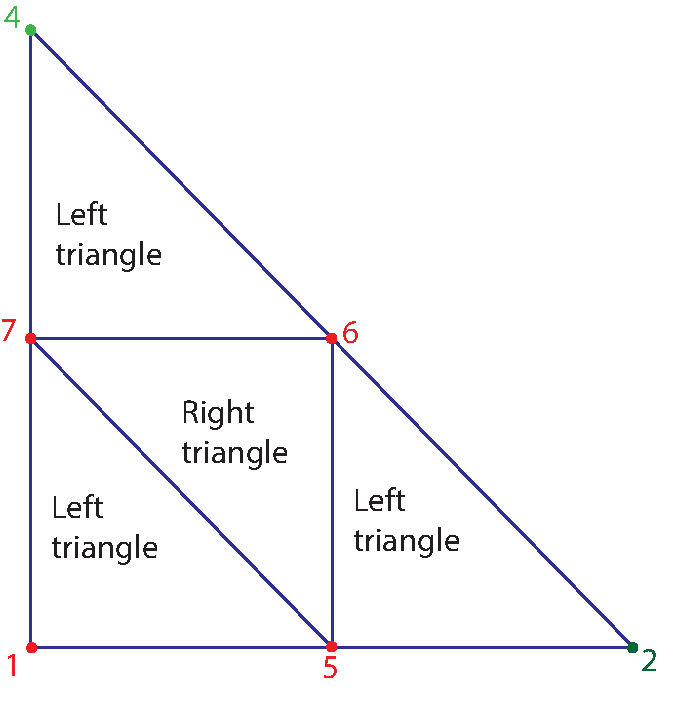
\includegraphics[width=0.95\textwidth]{Triangulation_left}
    \caption{Left triangulation refinement algorithm (recursive function L$\footnotesize{\textrm{EFT}}$ T$\footnotesize{\textrm{RIANGLE}}$).}
    \label{fig:triangulation_left}
\end{minipage}
\hfill
\begin{minipage}[t]{0.48\textwidth}
\centering
    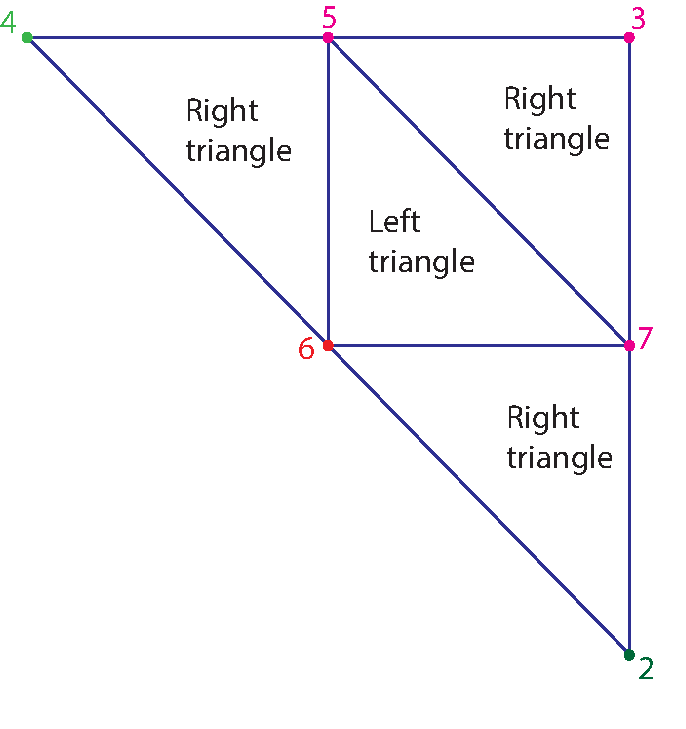
\includegraphics[width = 0.95\textwidth]{Triangulation_right}
    \caption{Right triangulation refinement algorithm (recursive function R$\footnotesize{\textrm{IGHT}}$ T$\footnotesize{\textrm{RIANGLE}}$).}
    \label{fig:triangulation_right}
\end{minipage}
\end{figure}
\begin{figure}[h]
  \begin{center}
  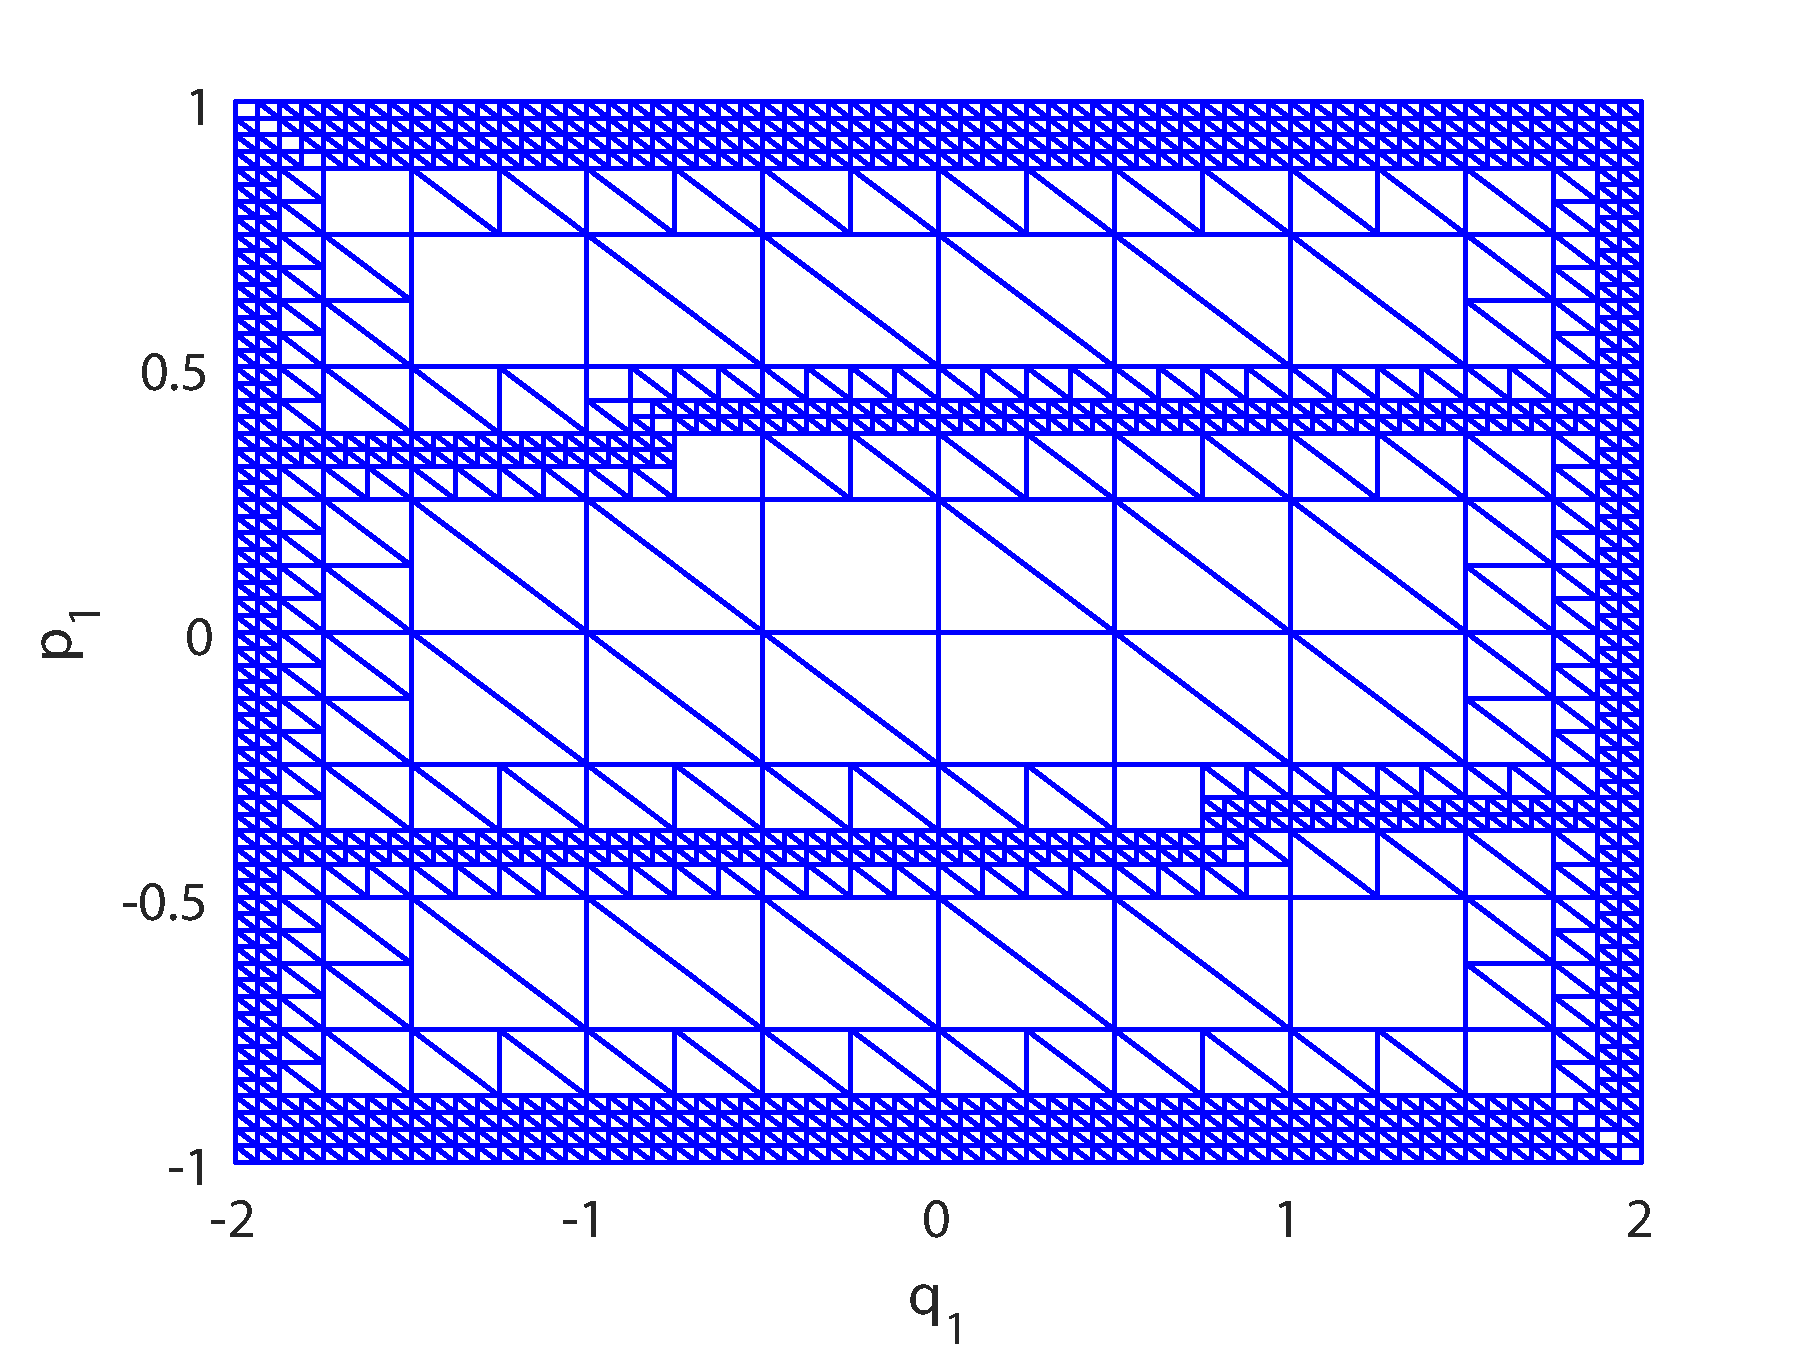
\includegraphics[width=\textwidth]{triangulation_source}
  \end{center}
  \caption{Triangulation refinement of source phase space:
  near the boundaries more rays are traced.
    The values of the parameters are $\varepsilon_{\variabile{q}_1^\textrm{min}}~=~ 0.1$ and $\varepsilon_{\variabile{q}_1^\textrm{max}}~=~1$.}
   \label{fig:triangulation_refinement}
  \end{figure}
\\ \indent The triangulation refinement allows finding \textit{all} the possible paths $(\Pi_\variabile{j})_{\variabile{j} = 1, \cdots, \npath}$ are their corresponding regions \set{R}{\textrm{s}}{}$(\Pi_\variabile{j})_{\variabile{j} = 1, \cdots, \npath}$. Using the edge-ray principle, we conclude that also the regions \set{R}{\textrm{t}}{}$(\Pi_\variabile{j})_{\variabile{j} = 1, \cdots, \npath}$ at the target are determined and only the rays close to the boundaries
$\partial$\set{R}{\textrm{s}}{} need to be considered to obtain the target ray distribution.
\section{Conclusions}
In this chapter we introduced the phase space concept. 
We explained a new ray tracing method based on the source and the target PS representation. 
In PS every point corresponds to a unique ray. 
The coordinates of every point correspond to the initial ray position $\variabile{q}_1$ and the initial ray direction $\variabile{p}_1 = \sin(\myangle_1)$ (expressed with respect to the normal of the source). The method also takes into account the paths followed by every ray traced.
Considering only reflection, every single ray follows only one path and, therefore, the PS regions do not overlap. 
\\ \indent
As an example, we provided the source and the target PS representation of the two-faceted cup.
The edge-ray principle guarantees that all the rays that follow the same path are located in the same regions in PS. If we know these regions at the source we can determine the corresponding regions at the target. 
It is sufficient to map the boundaries at the source $\partial$\set{R}{\textrm{s}}{}$(\Pi)$ to obtain their corresponding target boundaries $\partial$\set{R}{\textrm{t}}{}$(\Pi)$. \\ \indent
The boundaries $\partial$\set{R}{\textrm{t}}{}$(\Pi)$ are particularly relevant because there the luminance jumps from $0$ to a positive value. 
Assuming a Lambertian source, only the rays at the boundaries are needed to compute the target intensity. 
Based on this idea, a triangulation in \set{S}{}{} is constructed such that the rays closest to $\partial$\set{R}{\textrm{s}}{}$(\Pi)$
are selected and more rays in their vicinity are created to get progressively better estimates of the boundaries.
\\ \indent In Figures \ref{fig:three_distributions} we show three different ray distributions on the source PS of the two-faceted cup. In Figure \ref{fig:mc_sample}, $10^3$ random points are shown. MC ray tracing is based on this random distribution of the initial rays set. In Figure \ref{fig:qmc_sample}, $10^3$ points of a two-dimensional Sobol sequence are shown. 
Since Sobol sequences are defined in a unit square, we scaled it such that all the source PS \set{S}{}{}$=[-2, 2]\times[-1, 1]$ is covered by rays. Such regular distribution can lead to several advantages for the computation of the target intensity, see Section \ref{sec:QMC}. Finally, Figure \ref{fig:ps_sample} shows a non-uniform distribution of rays at the source PS on which PS ray tracing is based. Such distribution is obtained from the triangulation refinement explained in the previous section. The procedure requires tracing more rays close to the boundaries $\partial$\set{R}{\textrm{s}}{}$(\Pi)$ and only few rays in their interior.of the regions in source PS. 
From the edge ray-principle, we obtain that these rays will be located close to the boundaries $\partial$\set{R}{\textrm{t}}{}$(\Pi)$ of the regions at the target PS.
\\ \indent The target PS intensity is calculated using only the rays that are located at the boundaries $\partial$\set{R}{\textrm{t}}{}$(\Pi)$. Thus, in order to obtain the intensity profile at the target, the boundaries $\partial$\set{R}{\textrm{t}}{}$(\Pi)$ need to be determined.\\ \indent 
In the next chapter we provide two different approaches to find the boundaries $\partial$\set{R}{\textrm{t}}{}$(\Pi)$ using a set of rays given by the triangulation refinement.
\begin{figure}[h]
 \begin{subfigure}[t]{\textwidth}
\centering
    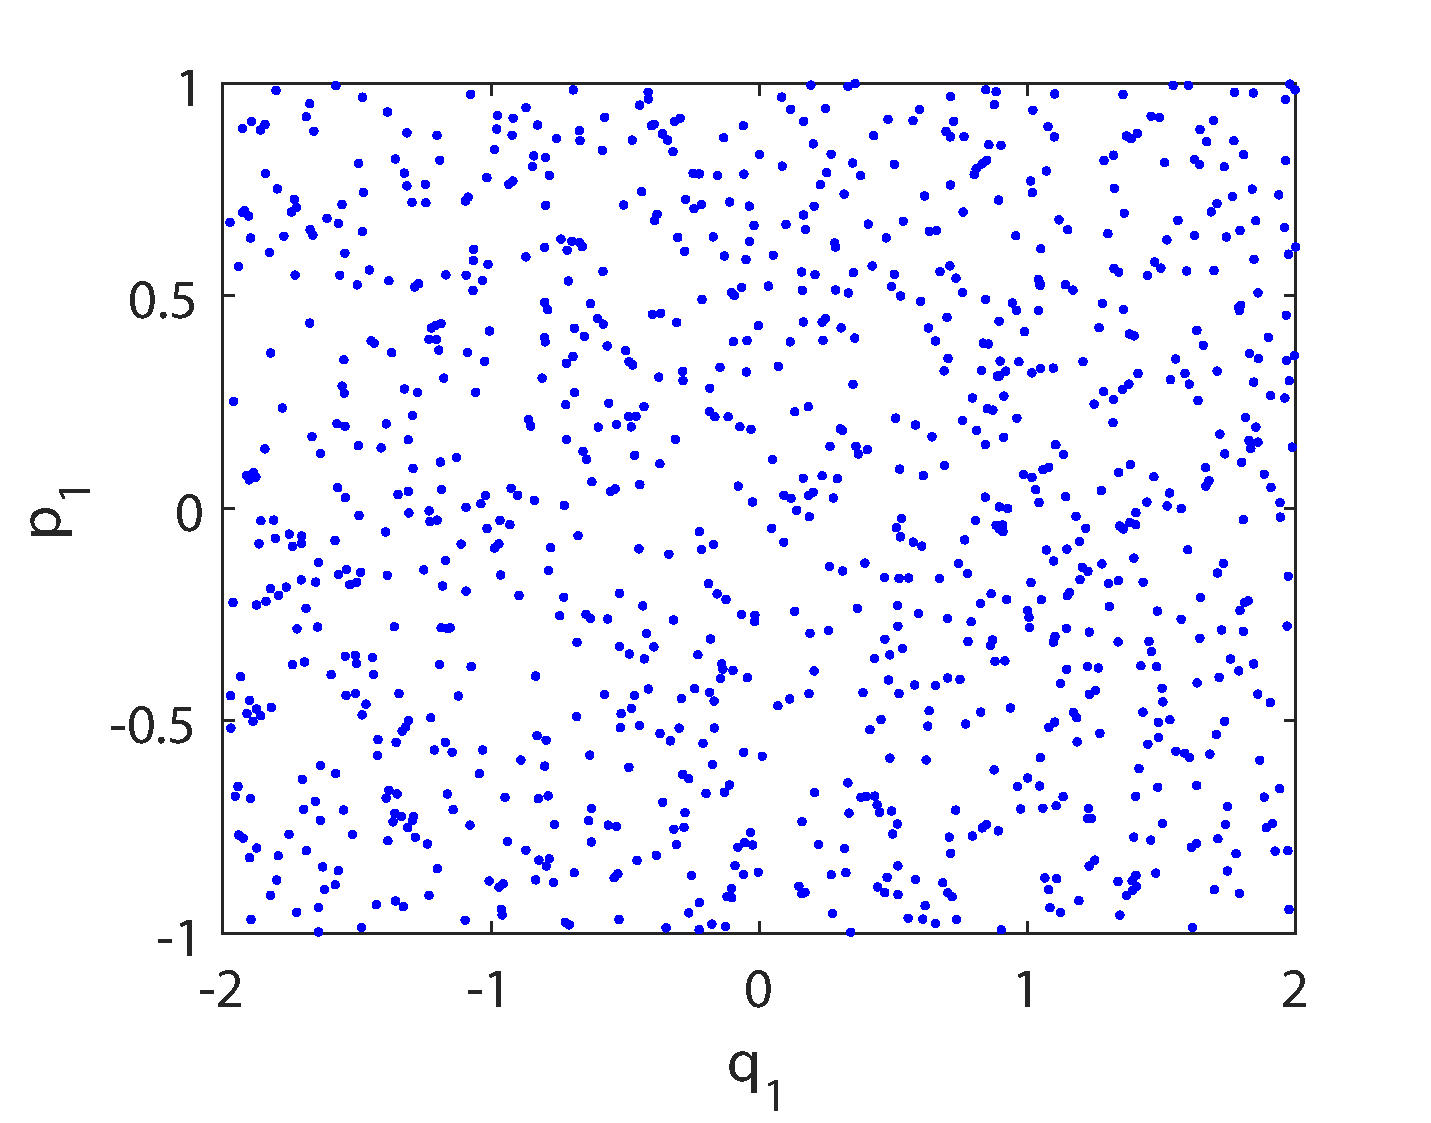
\includegraphics[width=0.57\textwidth]{MC_source_cup}
    \caption{$10^3$ random rays at the source PS (MC ray tracing).}
    \label{fig:mc_sample}
\end{subfigure}
\hfill
\\
\begin{subfigure}[t]{\textwidth}
\centering
    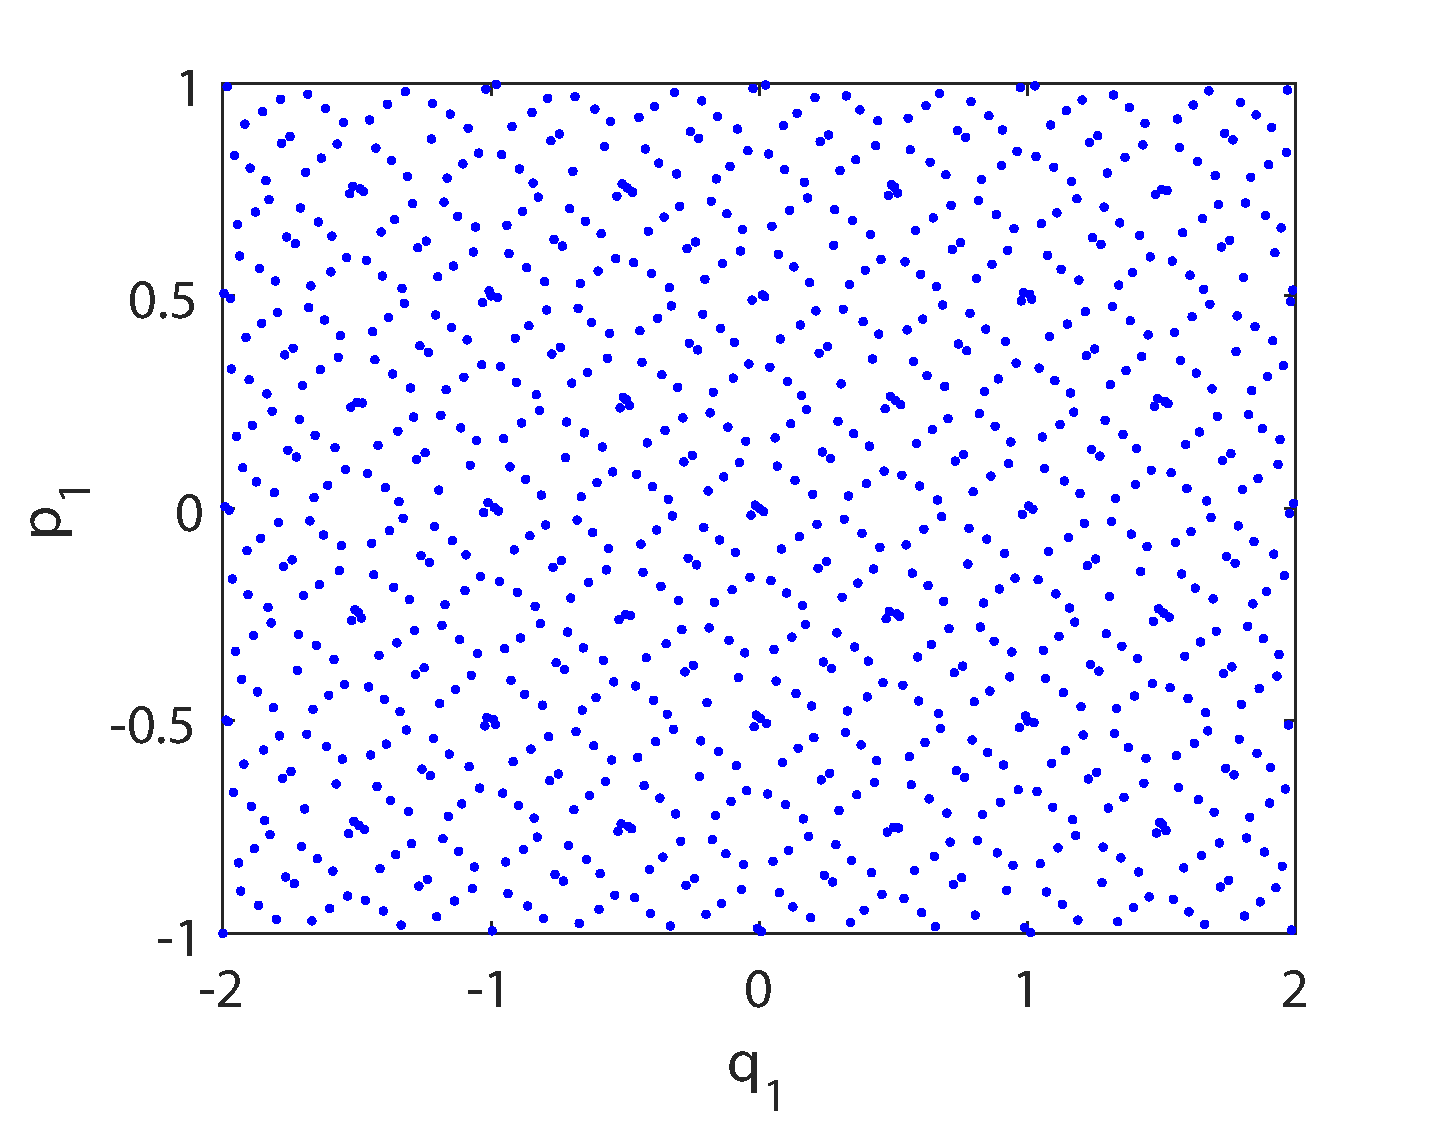
\includegraphics[width = 0.57\textwidth]{QMC_source_cup}
    \caption{$10^3$ rays at the source PS distributed as the point of a Sobol sequence (QMC ray tracing).}
    \label{fig:qmc_sample}
\end{subfigure}
\hfill
\begin{subfigure}[t]{\textwidth}
\centering
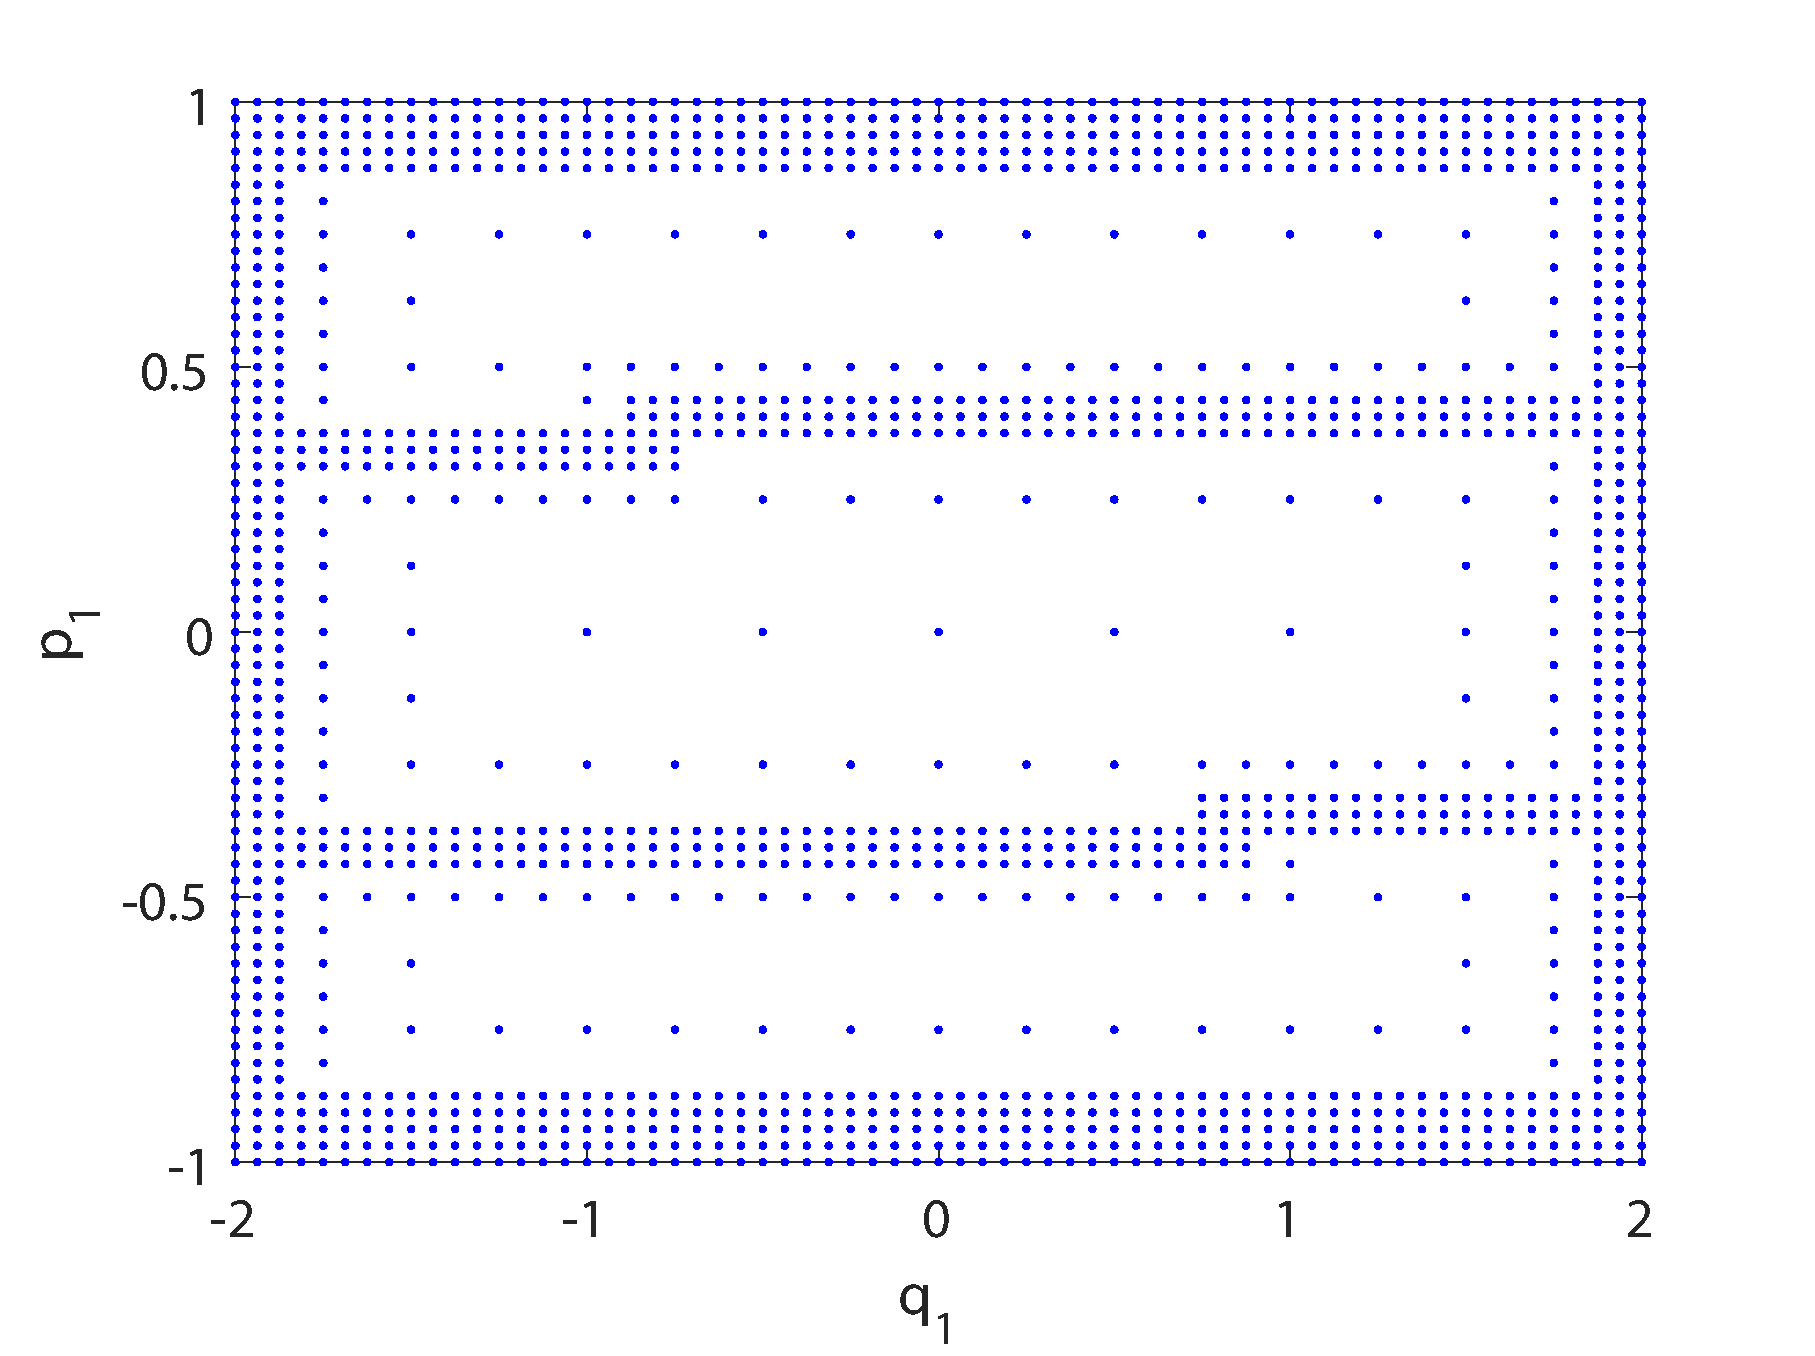
\includegraphics[width=0.57\textwidth]{PS_source_cup}
\caption{$1.5\cdot10^3$ rays distributed using the triangulation refinement (PS ray tracing).}
\label{fig:ps_sample}
\end{subfigure}
\caption{Three different ray distributions at the source of the two-faceted cup.}
\label{fig:three_distributions}
\end{figure}

% Compare all the PS
% Definition of luminance intensity and etendue
%\indent A similar method as described in this chapter is presented by Moore, \cite{moore2013methods}. In Moore's method each ray leaves the source at the same position while the angle coordinate changes. The path followed by the rays is taken into account and an interpolation is required to finalize the illumination pattern.
% This interpolation can affect the efficiency of the method. Our method employs the distribution of the rays at the target phase space and avoids using any interpolation.
%Moreover, a criterion to stop the algorithm is provided in such a way that no more rays than necessary are traced. This makes ray tracing in phase space more accurate compared with Moore's procedure.
% Finally, we claim that PS ray tracing is also more accurate than the ray tracing procedure proposed by Moore (2013), \cite{moore2013methods}.
%The novelty of our approach compared to the method used by Moore, is briefly explained below.
%First, to compute the output intensity, we employ the phase space of the target. This avoids the use of any interpolation to compute the photometric variables and therefore, more accurate results are obtained.
%Second, in \cite{moore2013methods} all rays that leave the source start at the same position and only a sampling angular range is given. In our approach a rectangular source is considered thus, both the angular and spatial coordinates of each ray change. This extra variable can produce very irregular shapes of the regions at target phase space. To overcome this issue, we employ the edge-ray principle and we consider the regions at source phase space where the distribution of the rays is much more regular and the corresponding boundaries are easily computed.
%As a consequence, our procedure is suitable to compute the output intensity as function of both the angular or the spatial coordinates.


% We need to compute the boundaries, explained in next chapter
